% !TeX program = xelatex
\documentclass[12pt, a4paper]{article}
\usepackage{amsmath}
\usepackage{xeCJK}
\usepackage{amsmath}
\usepackage{amssymb}
\usepackage{xcolor}
\usepackage{parskip}
\usepackage{tikz}

\setmainfont{Latin Modern Roman}
\setCJKmainfont{Noto Serif CJK TC}

\title{Ch1. to CH.4 High Light}

\begin{document}
\section*{Signal}
\subsection*{Signal Energy and Power}
\textbf{Continuous time}
\begin{align*}
	E_x &= \lim_{T \to \infty} \int_{-T}^{T} \mid x(t) \mid^2 dt = \int_{-\infty}^{\infty} \mid x(t) \mid^2 dt \quad \in(0, \infty) \\
	P_x &= \lim_{T \to \infty} \frac{1}{2T} \int_{-T}^{T} \mid x(t) \mid^2 dt \quad \in (0, \infty)
\end{align*}

\textbf{Discrete time}
\begin{align*}
	E_x &= \sum_{n=-\infty}^{\infty} \mid x[n] \mid^2 \quad \in (0, \infty) \\
	P_x &= \lim_{N \to \infty} \frac{1}{2N+1} \sum_{n = -N}^{N} \mid x[n] \mid^2 \quad \in(0, \infty)
\end{align*}

\subsection*{Periodic}
利用作圖看是不是週期訊號 \\
\textbf{當訊號為 Discrete time時}滿足週期比較嚴格,一定要在點上面,\color{red}並非\color{black}所有的$\cos$都是週期訊號,一定要符合$\omega_0N = 2\pi m$

\subsection*{Even and Odd Signals}
\begin{align*}
	\varepsilon_v \{ x(t) \} &= \frac {1}{2} [x(t) + x(-t)] \\
	O_v \{ x(t) \} &= \frac {1}{2} [x(t) - x(-t)] \\
\end{align*}
\newpage

\section*{Unit impulse and unit step functions}
\subsection*{Unit impulse}
\textbf{Continous time} \\
Unit impulse 在連續 $t=0$ 的時是 $\infty$,但積分後是1 $\to$ $\int \delta(t) \text{d}t = 1$
$$
\delta(t) = 
\begin{cases}
0, & t \ne 0 \\
\infty, & t = 0
\end{cases}
$$

\textbf{Discrete time} \\
Unit impulse 在離散 $n=0$ 的時候是1,其他時候是0
$$
\delta[n] = 
\begin{cases}
0, & n \ne 0 \\
1, & n = 0
\end{cases}
$$
\subsection*{Unit step function}
$$
u[n] = 
\begin{cases}
0, & n < 0 \\
1, & n \ge 0
\end{cases}
$$
$$
u(t) = 
\begin{cases}
0, & t < 0 \\
1, & t \ge 0
\end{cases}
$$
\subsection*{Proof $\int \delta(t) \text{d}t =1$}
$$
\delta(t) = 
\begin{cases}
\frac{1}{\Delta}, & 0 \le t \le \Delta \\
0
\end{cases}
$$
$$
\int_{0}^{\Delta} \delta_{\Delta}(t) \text{d}t = 1
$$
Therefore
$$
\delta(t) = \lim_{\Delta \to0}
\begin {cases}
\infty, & t = 0 \\
0, & t \ne 0
\end {cases}
$$
$$
\int_{0^-}^{0^+} \delta(t) \text{d}t = 1
$$
\newpage

\section*{System Properties}
\subsection*{Memoryless}
Input 的時序必須和 Output 的時序\textbf{完全一模一樣},不能有過去及未來。
$$
y(t) = [x(t) + x(t)^2]^2
$$
\subsection*{Invertibility}
這比較難一點,需要找出 Inverse system。或是可以從找出兩個不同的 Input 但是有相同的 Output 的反例來判斷。
\subsection*{Causulity}
Output 只和過去的 Input 有關。看他的時間只要沒跟未來有關就是 Causlity。
\subsection*{Stability}
使用 BIBO(Bounded Input Bounded Output) 來判斷,若 Input 為有限值, Output 也是有限值,則這個系統 Stable。\\
\textit{Example:}
\begin{align*}
	&y[n] = x[n-1] \\
	&\left| x[n] \right| < B \to \left|y[n] \right| = \left| x[n-1] \right| < B < \infty
\end{align*}
\subsection*{Linear}
線性系統的特性是 superposition,所以可以使用 $x_1 \to y1$, $x_2 \to y2$ 然後令 $x_3 = \alpha x_1 + \beta x_2$ 看 $y_3$ 是否等於 $\alpha y_1 + \beta y_2$,若成立,則此系統為 linear。
\subsection*{Time-Invarient}
非時變系統是相同的 Input 不會隨著輸入時間的不同,而有不同的 Output。利用將 Input 向右平移 $t_0$(延遲 $t_0$)看 Output 是否也向右平移 $t_0$(延遲 $t_0$)來判斷是否為 time-invarient。
\newpage

\section*{LTI(Linear Time-Invariant) Systems}
LTI system 是先將 $\delta$ 函數丟入 system 產生對應的響應 $h$ 然後將 input 和 h 做 convolution 就可以得到 input 丟入系統所對應的output
\begin{center}
\tikzset{every picture/.style={line width=0.75pt}} %set default line width to 0.75pt        

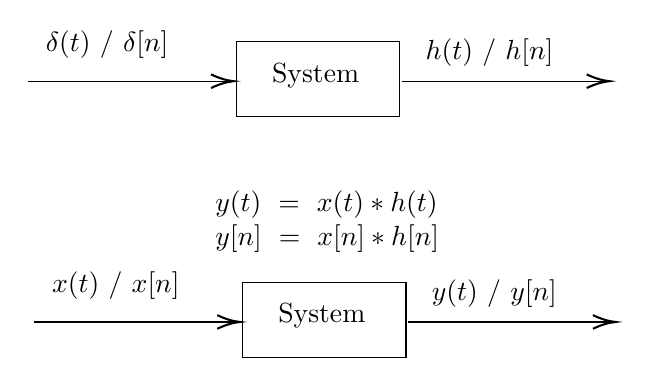
\begin{tikzpicture}[x=0.75pt,y=0.75pt,yscale=-1,xscale=1]
%uncomment if require: \path (0,300); %set diagram left start at 0, and has height of 300

%Shape: Rectangle [id:dp4204380002688358] 
\draw   (297,99.92) -- (375.77,99.92) -- (375.77,135.92) -- (297,135.92) -- cycle ;
%Straight Lines [id:da23613823984617388] 
\draw    (196.77,118.92) -- (293.77,118.92) ;
\draw [shift={(295.77,118.92)}, rotate = 180] [color={rgb, 255:red, 0; green, 0; blue, 0 }  ][line width=0.75]    (10.93,-3.29) .. controls (6.95,-1.4) and (3.31,-0.3) .. (0,0) .. controls (3.31,0.3) and (6.95,1.4) .. (10.93,3.29)   ;
%Straight Lines [id:da6308882612547787] 
\draw    (376.77,118.92) -- (474.77,118.92) ;
\draw [shift={(476.77,118.92)}, rotate = 180] [color={rgb, 255:red, 0; green, 0; blue, 0 }  ][line width=0.75]    (10.93,-3.29) .. controls (6.95,-1.4) and (3.31,-0.3) .. (0,0) .. controls (3.31,0.3) and (6.95,1.4) .. (10.93,3.29)   ;
%Shape: Rectangle [id:dp5949065708697123] 
\draw   (300,215.92) -- (378.77,215.92) -- (378.77,251.92) -- (300,251.92) -- cycle ;
%Straight Lines [id:da4813794065172372] 
\draw    (199.77,234.92) -- (296.77,234.92) ;
\draw [shift={(298.77,234.92)}, rotate = 180] [color={rgb, 255:red, 0; green, 0; blue, 0 }  ][line width=0.75]    (10.93,-3.29) .. controls (6.95,-1.4) and (3.31,-0.3) .. (0,0) .. controls (3.31,0.3) and (6.95,1.4) .. (10.93,3.29)   ;
%Straight Lines [id:da1899703445501454] 
\draw    (379.77,234.92) -- (477.77,234.92) ;
\draw [shift={(479.77,234.92)}, rotate = 180] [color={rgb, 255:red, 0; green, 0; blue, 0 }  ][line width=0.75]    (10.93,-3.29) .. controls (6.95,-1.4) and (3.31,-0.3) .. (0,0) .. controls (3.31,0.3) and (6.95,1.4) .. (10.93,3.29)   ;

% Text Node
\draw (313,109) node [anchor=north west][inner sep=0.75pt]   [align=left] {System};
% Text Node
\draw (204,93.4) node [anchor=north west][inner sep=0.75pt]    {$\delta ( t) \ /\ \delta [ n]$};
% Text Node
\draw (387,97.4) node [anchor=north west][inner sep=0.75pt]    {$h( t) \ /\ h[ n]$};
% Text Node
\draw (316,225) node [anchor=north west][inner sep=0.75pt]   [align=left] {System};
% Text Node
\draw (207,209.4) node [anchor=north west][inner sep=0.75pt]    {$x( t) \ /\ x[ n]$};
% Text Node
\draw (390,213.4) node [anchor=north west][inner sep=0.75pt]    {$y( t) \ /\ y[ n]$};
% Text Node
\draw (279,169.4) node [anchor=north west][inner sep=0.75pt]    {$ \begin{array}{l}
y( t) \ =\ x( t) *h( t)\\
y[ n] \ =\ x[ n] *h[ n]
\end{array}$};
\end{tikzpicture}
\end{center}
\subsection*{Convolution}
\textbf{Continous time}
$$
y(t) = x(t)*h(t) = \int_{-\infty}^{\infty} x(\tau)h(t-\tau)\text{d}\tau
$$
\textbf{Discrete time}
$$
y[n] = x[n]*h[n] = \sum_{k=-\infty}^{\infty} x[k]h[n-k]
$$
\subsection*{Important equivlent}
\textbf{Discrete time}
\begin{align*}
	x[n] &= x[n]*\delta[n] \\
	x[n+k] &= x[n]*\delta[n+k] \\
\end{align*}
\textbf{Continous time}
\begin{align*}
	x(t) &= x(t)*\delta(t) \\
	x(t+k) &= x(t)*\delta(t+k)
\end{align*}


\subsection*{Properties of convoluation}
\subsubsection*{Commutative}
\textbf{Discrete time} $x[n]*h[n] = h[n]*x[n]$
$$
\sum_{k=-\infty}^{\infty} x[k]h[n-k] = \sum_{k=-\infty}^{\infty} h[k]x[n-k]
$$
\textbf{Continous time} $x(t)*h(t) = h(t)*x(t)$
$$
\int_{-\infty}^{\infty} x(\tau)h(t-\tau)\text{d}\tau = \int_{-\infty}^{\infty} h(\tau)x(t-\tau)\text{d}\tau
$$

\subsubsection*{Distributive}
\textbf{Discrete time} $x[n]*(h_1[n] + h_2[n]) = x[n]*h_1[n] + x[n]*h_2[n]$ \\
\textbf{Continous time} $x(t)*(h_1(t) + h_2(t)) = x(t)*h_1(t) + x(t)*h_2(t)$

\subsubsection*{Additive(Linear)}
\textbf{Discrete time} $(x_1[n]+x_2[n])*h[n] = x_1[n]*h[n] + x_2[n]*h[n]$ \\
\textbf{Continous time} $(x_1(t)+x_2(t))*h(t) = x_1(t)*h(t) + x_2(t)*h(t)$

\subsubsection*{Associative}
\textbf{Discrete time} $x[n]*(h_1[n]*h_2[n]) = (x[n]*h_1[n])*h_2[n]$ \\
\textbf{Continous time} $x(t)*(h_1(t)*h_2(t)) = (x(t)*h_1(t))*h_2(t)$
\begin{center}


\tikzset{every picture/.style={line width=0.75pt}} %set default line width to 0.75pt        

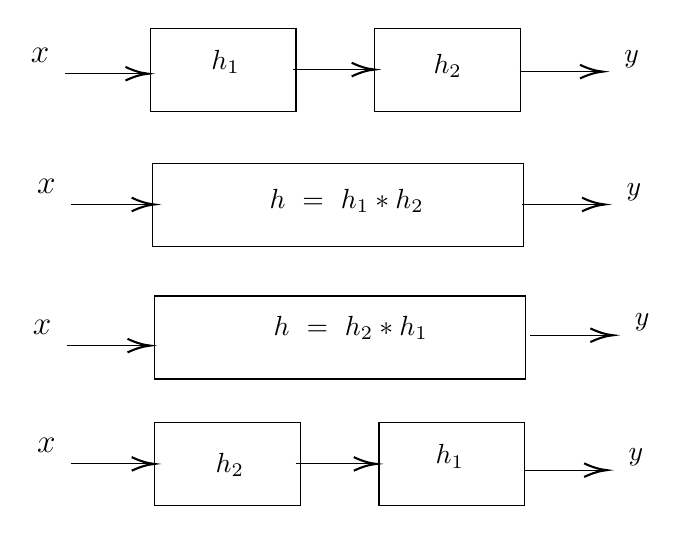
\begin{tikzpicture}[x=0.75pt,y=0.75pt,yscale=-1,xscale=1]
%uncomment if require: \path (0,300); %set diagram left start at 0, and has height of 300

%Shape: Rectangle [id:dp8805200523913231] 
\draw   (259,32) -- (329,32) -- (329,72) -- (259,72) -- cycle ;
%Shape: Rectangle [id:dp8235779632151183] 
\draw   (367,32) -- (437,32) -- (437,72) -- (367,72) -- cycle ;
%Shape: Rectangle [id:dp6359840555839769] 
\draw   (259.77,97) -- (438.77,97) -- (438.77,137) -- (259.77,137) -- cycle ;
%Shape: Rectangle [id:dp08006179479990161] 
\draw   (260.77,161) -- (439.77,161) -- (439.77,201) -- (260.77,201) -- cycle ;
%Shape: Rectangle [id:dp7700226635379218] 
\draw   (261,222) -- (331,222) -- (331,262) -- (261,262) -- cycle ;
%Shape: Rectangle [id:dp28557116730178933] 
\draw   (369,222) -- (439,222) -- (439,262) -- (369,262) -- cycle ;
%Straight Lines [id:da5761705109627222] 
\draw    (217.77,53.92) -- (255.77,53.92) ;
\draw [shift={(257.77,53.92)}, rotate = 180] [color={rgb, 255:red, 0; green, 0; blue, 0 }  ][line width=0.75]    (10.93,-3.29) .. controls (6.95,-1.4) and (3.31,-0.3) .. (0,0) .. controls (3.31,0.3) and (6.95,1.4) .. (10.93,3.29)   ;
%Straight Lines [id:da23176508793808637] 
\draw    (220.77,116.92) -- (258.77,116.92) ;
\draw [shift={(260.77,116.92)}, rotate = 180] [color={rgb, 255:red, 0; green, 0; blue, 0 }  ][line width=0.75]    (10.93,-3.29) .. controls (6.95,-1.4) and (3.31,-0.3) .. (0,0) .. controls (3.31,0.3) and (6.95,1.4) .. (10.93,3.29)   ;
%Straight Lines [id:da324493480437135] 
\draw    (218.77,184.92) -- (256.77,184.92) ;
\draw [shift={(258.77,184.92)}, rotate = 180] [color={rgb, 255:red, 0; green, 0; blue, 0 }  ][line width=0.75]    (10.93,-3.29) .. controls (6.95,-1.4) and (3.31,-0.3) .. (0,0) .. controls (3.31,0.3) and (6.95,1.4) .. (10.93,3.29)   ;
%Straight Lines [id:da6440074473499616] 
\draw    (220.77,241.92) -- (258.77,241.92) ;
\draw [shift={(260.77,241.92)}, rotate = 180] [color={rgb, 255:red, 0; green, 0; blue, 0 }  ][line width=0.75]    (10.93,-3.29) .. controls (6.95,-1.4) and (3.31,-0.3) .. (0,0) .. controls (3.31,0.3) and (6.95,1.4) .. (10.93,3.29)   ;
%Straight Lines [id:da11729276240151787] 
\draw    (327.77,51.92) -- (364.77,51.92) ;
\draw [shift={(366.77,51.92)}, rotate = 180] [color={rgb, 255:red, 0; green, 0; blue, 0 }  ][line width=0.75]    (10.93,-3.29) .. controls (6.95,-1.4) and (3.31,-0.3) .. (0,0) .. controls (3.31,0.3) and (6.95,1.4) .. (10.93,3.29)   ;
%Straight Lines [id:da5575163341209703] 
\draw    (328.77,241.92) -- (365.77,241.92) ;
\draw [shift={(367.77,241.92)}, rotate = 180] [color={rgb, 255:red, 0; green, 0; blue, 0 }  ][line width=0.75]    (10.93,-3.29) .. controls (6.95,-1.4) and (3.31,-0.3) .. (0,0) .. controls (3.31,0.3) and (6.95,1.4) .. (10.93,3.29)   ;
%Straight Lines [id:da22189195806400008] 
\draw    (436.77,52.92) -- (474.77,52.92) ;
\draw [shift={(476.77,52.92)}, rotate = 180] [color={rgb, 255:red, 0; green, 0; blue, 0 }  ][line width=0.75]    (10.93,-3.29) .. controls (6.95,-1.4) and (3.31,-0.3) .. (0,0) .. controls (3.31,0.3) and (6.95,1.4) .. (10.93,3.29)   ;
%Straight Lines [id:da9013427813386689] 
\draw    (437.77,116.92) -- (475.77,116.92) ;
\draw [shift={(477.77,116.92)}, rotate = 180] [color={rgb, 255:red, 0; green, 0; blue, 0 }  ][line width=0.75]    (10.93,-3.29) .. controls (6.95,-1.4) and (3.31,-0.3) .. (0,0) .. controls (3.31,0.3) and (6.95,1.4) .. (10.93,3.29)   ;
%Straight Lines [id:da40073295423463773] 
\draw    (441.77,179.92) -- (479.77,179.92) ;
\draw [shift={(481.77,179.92)}, rotate = 180] [color={rgb, 255:red, 0; green, 0; blue, 0 }  ][line width=0.75]    (10.93,-3.29) .. controls (6.95,-1.4) and (3.31,-0.3) .. (0,0) .. controls (3.31,0.3) and (6.95,1.4) .. (10.93,3.29)   ;
%Straight Lines [id:da6729366003239877] 
\draw    (438.77,244.92) -- (476.77,244.92) ;
\draw [shift={(478.77,244.92)}, rotate = 180] [color={rgb, 255:red, 0; green, 0; blue, 0 }  ][line width=0.75]    (10.93,-3.29) .. controls (6.95,-1.4) and (3.31,-0.3) .. (0,0) .. controls (3.31,0.3) and (6.95,1.4) .. (10.93,3.29)   ;

% Text Node
\draw (200,40.4) node [anchor=north west][inner sep=0.75pt]  [font=\large]  {$x$};
% Text Node
\draw (203,103.4) node [anchor=north west][inner sep=0.75pt]  [font=\large]  {$x$};
% Text Node
\draw (201,171.4) node [anchor=north west][inner sep=0.75pt]  [font=\large]  {$x$};
% Text Node
\draw (203,228.4) node [anchor=north west][inner sep=0.75pt]  [font=\large]  {$x$};
% Text Node
\draw (486,41.4) node [anchor=north west][inner sep=0.75pt]    {$y$};
% Text Node
\draw (487,105.4) node [anchor=north west][inner sep=0.75pt]    {$y$};
% Text Node
\draw (491,168.4) node [anchor=north west][inner sep=0.75pt]    {$y$};
% Text Node
\draw (488,233.4) node [anchor=north west][inner sep=0.75pt]    {$y$};
% Text Node
\draw (287,41.4) node [anchor=north west][inner sep=0.75pt]    {$h_{1}$};
% Text Node
\draw (394,43.4) node [anchor=north west][inner sep=0.75pt]    {$h_{2}$};
% Text Node
\draw (289,235.4) node [anchor=north west][inner sep=0.75pt]    {$h_{2}$};
% Text Node
\draw (395,231.4) node [anchor=north west][inner sep=0.75pt]    {$h_{1}$};
% Text Node
\draw (317,169.4) node [anchor=north west][inner sep=0.75pt]    {$h\ =\ h_{2} *h_{1}$};
% Text Node
\draw (315,108.4) node [anchor=north west][inner sep=0.75pt]    {$h\ =\ h_{1} *h_{2}$};
\end{tikzpicture}
\end{center}
\newpage

\subsection*{Properties of LTI system}
\subsubsection*{Memoryless / with Memory}
LTI system 只有在 $h[n] = k\delta[n]$ 或是 $h(t) = k\delta(t)$是\color{red} Memoryless \color{black},其他時候都是 \color{blue} with Memory \color{black}

\subsubsection*{Causality}
Causal 只會發生在$h[n] = 0$, for $n<0$ 或是 $h(t) = 0$, for $t<0$
\begin{align*}
	y[n] &= \sum_{k = -\infty}^{\infty} x[k]h[n-k] \\
			 &= \sum_{k = -\infty}^{\infty} h[k]x[n-k] \\
			 &= h[0]x[n] + h[1]x[n-1] + h[2]x[n-2] + ... &&\qquad \color{green} x[n-k] \color{black} \\
			 &+ h[-1]x[n+1] + h[-2]x[n+2] + h[-3]x[n+3] &&\qquad \color{red} x[n+k] \text{未來訊號} \color{black} \\
	y(t) &= \int_{-\infty}^{\infty} x(\tau)h(t-\tau)\text{d}\tau \\
			 &= \int_{-\infty}^{\infty} h(\tau)x(t-\tau)\text{d}\tau \\
			 &= \int_{-\infty}^{0} h(\tau) \color{red}\underbrace {\color{black}x(t-\tau)}_{\text{未來部分}}\color{black}\text{d}\tau + \int_{0}^{\infty} h(\tau) \color{green}\underbrace{\color{black}x(t-\tau)}_{\text{過去部分}}\color{black} \text{d}\tau
\end{align*}

\subsubsection*{Invertibility}
如果系統的 impulse response($h(t)$, $h[n]$) 是 invertible 則它有 LTI inverse impulse response ($h_I(t)$, $h_I[n]$) \\
\begin{align*}
	h(t)*h_I(t) &= \delta(t) \\
	h[n]*h_I[n] &= \delta[n]
\end{align*}
\begin{center}


\tikzset{every picture/.style={line width=0.75pt}} %set default line width to 0.75pt        

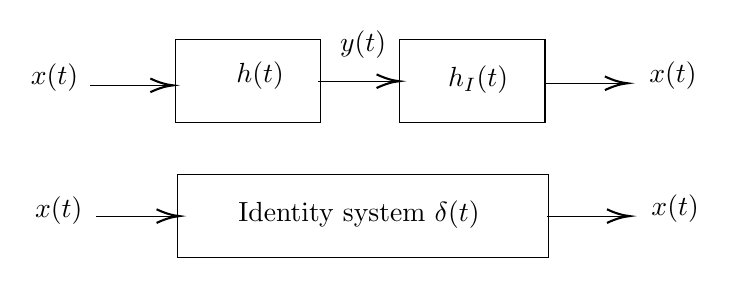
\begin{tikzpicture}[x=0.75pt,y=0.75pt,yscale=-1,xscale=1]
%uncomment if require: \path (0,300); %set diagram left start at 0, and has height of 300

%Shape: Rectangle [id:dp8805200523913231] 
\draw   (253,85) -- (323,85) -- (323,125) -- (253,125) -- cycle ;
%Shape: Rectangle [id:dp8235779632151183] 
\draw   (361,85) -- (431,85) -- (431,125) -- (361,125) -- cycle ;
%Shape: Rectangle [id:dp6359840555839769] 
\draw   (253.77,150) -- (432.77,150) -- (432.77,190) -- (253.77,190) -- cycle ;
%Straight Lines [id:da5761705109627222] 
\draw    (211.77,106.92) -- (249.77,106.92) ;
\draw [shift={(251.77,106.92)}, rotate = 180] [color={rgb, 255:red, 0; green, 0; blue, 0 }  ][line width=0.75]    (10.93,-3.29) .. controls (6.95,-1.4) and (3.31,-0.3) .. (0,0) .. controls (3.31,0.3) and (6.95,1.4) .. (10.93,3.29)   ;
%Straight Lines [id:da23176508793808637] 
\draw    (214.77,169.92) -- (252.77,169.92) ;
\draw [shift={(254.77,169.92)}, rotate = 180] [color={rgb, 255:red, 0; green, 0; blue, 0 }  ][line width=0.75]    (10.93,-3.29) .. controls (6.95,-1.4) and (3.31,-0.3) .. (0,0) .. controls (3.31,0.3) and (6.95,1.4) .. (10.93,3.29)   ;
%Straight Lines [id:da11729276240151787] 
\draw    (321.77,104.92) -- (358.77,104.92) ;
\draw [shift={(360.77,104.92)}, rotate = 180] [color={rgb, 255:red, 0; green, 0; blue, 0 }  ][line width=0.75]    (10.93,-3.29) .. controls (6.95,-1.4) and (3.31,-0.3) .. (0,0) .. controls (3.31,0.3) and (6.95,1.4) .. (10.93,3.29)   ;
%Straight Lines [id:da22189195806400008] 
\draw    (430.77,105.92) -- (468.77,105.92) ;
\draw [shift={(470.77,105.92)}, rotate = 180] [color={rgb, 255:red, 0; green, 0; blue, 0 }  ][line width=0.75]    (10.93,-3.29) .. controls (6.95,-1.4) and (3.31,-0.3) .. (0,0) .. controls (3.31,0.3) and (6.95,1.4) .. (10.93,3.29)   ;
%Straight Lines [id:da9013427813386689] 
\draw    (431.77,169.92) -- (469.77,169.92) ;
\draw [shift={(471.77,169.92)}, rotate = 180] [color={rgb, 255:red, 0; green, 0; blue, 0 }  ][line width=0.75]    (10.93,-3.29) .. controls (6.95,-1.4) and (3.31,-0.3) .. (0,0) .. controls (3.31,0.3) and (6.95,1.4) .. (10.93,3.29)   ;

% Text Node
\draw (182,95.4) node [anchor=north west][inner sep=0.75pt]  [font=\normalsize]  {$x( t)$};
% Text Node
\draw (184,159.4) node [anchor=north west][inner sep=0.75pt]  [font=\normalsize]  {$x( t)$};
% Text Node
\draw (480,94.4) node [anchor=north west][inner sep=0.75pt]    {$x( t)$};
% Text Node
\draw (481,158.4) node [anchor=north west][inner sep=0.75pt]    {$x( t)$};
% Text Node
\draw (281,94.4) node [anchor=north west][inner sep=0.75pt]    {$h( t)$};
% Text Node
\draw (383,96.4) node [anchor=north west][inner sep=0.75pt]    {$h_{I}( t)$};
% Text Node
\draw (282,161.4) node [anchor=north west][inner sep=0.75pt]    {$\text{Identity system } \delta ( t)$};
% Text Node
\draw (331,79.4) node [anchor=north west][inner sep=0.75pt]    {$y( t)$};
\end{tikzpicture}
\end{center}
\newpage

\subsubsection*{Stability}
\textbf{Discrete time:} given bounded input $\left|x[n]\right|<B$, for all $n$ \\
magnitude of the output is
\begin{align*}
	\left|y[n]\right| &= \left|\sum_{k=-\infty}^{\infty}h[k]x[n-k]\right| \\
										&\leq \sum_{k=-\infty}^{\infty}\left|h[k]\right| \cdot \left|x[n-k]\right| \\
										&\leq B \sum_{k=-\infty}^{\infty} \left|h[k]\right|
\end{align*}
The impulse response is absolutely summable that
$$
\sum_{k=-\infty}^{\infty} \left|h[k]\right|<\infty
$$
\\ \\
\textbf{Continous time:} given bounded input $\left|x(t)\right|<B$, for all $t$ \\
magnitude of the output is
\begin{align*}
	\left|y(t)\right| &= \left|\int_{-\infty}^{\infty}h(\tau)x(t-\tau)\text{d}\tau\right|\\
										&\leq \int_{-\infty}^{\infty}\left|h(\tau)\right|\cdot\left|x(t-\tau)\right| \text{d}\tau \\
										&\leq B\int_{-\infty}^{\infty}\left|h(\tau)\right|\text{d}\tau
\end{align*}
The impulse response is absolutely summable that
$$
\int_{-\infty}^{\infty} \left|h(\tau)\right|<\infty
$$
\newpage

\subsection*{Singularity Functions}
\subsubsection*{Differentiator}
Unit impulse response of a diffrentiator
$$
h(t) = \frac{\text{d}\delta(t)}{\text{d}t} \equiv u_1'(t)
$$
Convolution will be 
$$
\frac{\text{d}x(t)}{\text{d}t}= x(t)*u_1'(t)
$$
\textbf{\textit{pf.}}
\begin{align*}
	\frac{\text{d}x(t)}{\text{d}t} &= \lim_{\Delta t \to 0} \frac{x(t)-x(t-\Delta t)}{\Delta t} \\
																 &= \lim_{\Delta t \to 0} \frac{x(t)*(\color{red}\delta(t)-\delta(t-\Delta t)\color{black})}{\Delta t} \\
																 &= x(t) * \color{red} \frac{\delta(t)}{\text{d}t} \color{black}
\end{align*}

\subsubsection*{Integrator}
Unit impulse response of a diffrentiator
$$
h(t) = \int_{-\infty}^{t}\delta(\tau)\text{d}\tau \equiv u(t)
$$
Convolution will be 
$$
x(t)*u(t) = \int_{-\infty}^{\infty}x(\tau)u(t-\tau)\text{d}\tau = \int_{-\infty}^{t}x(t)\text{d}\tau
$$
\newpage

\section*{Fourier Series Representation}
\subsection*{Continous time}
\begin{align*}
	x(t) &= \sum_{k=-\infty}^{\infty}a_ke^{jk\omega_0t}\\
	a_k &= \frac{1}{T} \int_T x(t) \cdot e^{-jk\omega_0t} \text{d}t
\end{align*}
$a_k$ 就是將 $x(t)$ 對基底$e^{jk\omega_0t}$ 用內積得到投影的長度,因為複數內積要取 conjugate 所以會有負號,連續的 $\omega_0 = 2\pi / T$
\subsubsection*{Properties}

\begin{center}
	\begin{tabular} { |c|c c| }
		\hline
		Property & Periodic Signal & Fourier Series Coefficients \\
		\hline
		Linearty & $Ax(t) + By(t)$ & $Aa_k + Bb_k$ \\
		Time Shifting & $t-t_0$ & $a_ke^{-jk\omega_0t_0}$ \\
		Frequency Shifting & $e^{jM\omega_0t}x(t)$ & $a_{k-M}$ \\
		Conjugation & $x^*(t)$ & $a^*_{-k}$ \\
		Multiplication & $x(t)y(t)$ & $\sum_{l=-\infty}^{\infty}a_l b_{k-l}$ \\
		Differentiation & $\frac{\text{d}x(t)}{\text{d}t}$ & $jk\omega_0a_k$ \\
		Integration & $\int_{-\infty}^{t}x(t)\text{d}t$ & $\left(\frac{1}{jk\omega_0}\right)a_k$ \\
		\hline
	\end{tabular}
\end{center}
Conjugate symmetry for real signals($x(t)$ is real)
\begin{align*}
	\begin{cases}
		a_k = a^*_{-k} \\
		\Re \{a_k\} = \Re \{a_{-k}\} \\
		\Im  \{a_k\} = -\Im \{a_{-k}\} \\
		\left|a_k\right| = \left|a_{-k}\right| \\
		\angle a_k = -\angle a_k
	\end{cases}
\end{align*}

\begin{minipage}[t]{0.3 \textwidth}
\begin{align*}
	\begin{cases}
	  x_e(t) = Ev \{x(t)\} \\
		x_o(t) = Od \{x(t)\}
	\end{cases}
\end{align*}
\end{minipage}
\hfill
\begin{minipage}[t]{0.3 \textwidth}
\begin{align*}
	\begin{cases}
		\Re \{a_k\} \\
	  j\Im \{a_k\}	\\
\end{cases}
\end{align*}
\end{minipage}
\\ \\
Parseval's Relation
$$
\frac{1}{T} \int_T \left|x(t)\right|^2 \text{d}t = \sum_{k=-\infty}^{\infty} \left|a_k\right|^2
$$
\newpage

\subsection*{Discrete time}
\begin{align*}
	x[n] &= \sum_{k=\langle N \rangle}a_ke^{jk\omega_0n}\\
	a_k &= \frac{1}{N} \sum_{n=\langle N \rangle} x[n] \cdot e^{-jk\omega_0n}
\end{align*}
$a_k$ 就是將 $x[n]$ 對基底$e^{jk\omega_0n}$ 用內積得到投影的長度,因為複數內積要取 conjugate 所以會有負號,離散的 $\omega_0 = 2\pi / N$
\subsubsection*{Properties}

\begin{center}
	\begin{tabular} { |c|c c| }
		\hline
		Property & Periodic Signal & Fourier Series Coefficients \\
		\hline
		Linearty & $Ax[n] + By[n]$ & $Aa_k + Bb_k$ \\
		Time Shifting & $n-n_0$ & $a_ke^{-jk\omega_0n_0}$ \\
		Frequency Shifting & $e^{jM\omega_0t}x[n]$ & $a_{k-M}$ \\
		Conjugation & $x^*[n]$ & $a^*_{-k}$ \\
		Multiplication & $x[n]y[n]$ & $\sum_{l=-\infty}^{\infty}a_l b_{k-l}$ \\
		First Difference & $x[n] - x[n-1]$ & $(1-e^{-jk\omega_0})a_k$ \\
		Running Sum & $\sum_{k = -\infty}^{n} x[k]$ & $\left(\frac{1}{1-e^{-jk\omega_0}}\right)a_k$ \\
		\hline
	\end{tabular}
\end{center}
Conjugate symmetry for real signals($x(t)$ is real)
\begin{align*}
	\begin{cases}
		a_k = a^*_{-k} \\
		\Re \{a_k\} = \Re \{a_{-k}\} \\
		\Im  \{a_k\} = -\Im \{a_{-k}\} \\
		\left|a_k\right| = \left|a_{-k}\right| \\
		\angle a_k = -\angle a_k
	\end{cases}
\end{align*}

\begin{minipage}[t]{0.3 \textwidth}
\begin{align*}
	\begin{cases}
	  x_e(t) = Ev \{x(t)\} \\
		x_o(t) = Od \{x(t)\}
	\end{cases}
\end{align*}
\end{minipage}
\hfill
\begin{minipage}[t]{0.3 \textwidth}
\begin{align*}
	\begin{cases}
		\Re \{a_k\} \\
	  j\Im \{a_k\}	\\
\end{cases}
\end{align*}
\end{minipage}
\\ \\
Parseval's Relation
$$
\frac{1}{N} \sum_{n = \langle N \rangle} \left|x(t)\right|^2 \text{d}t = \sum_{k=\langle N \rangle} \left|a_k\right|^2
$$
\newpage

\subsection*{With LTI system}
\textbf{Continuous time} \\
Let $H(j\omega)$ as frequency response of the system
$$
H(j\omega) = \int_{-\infty}^{\infty} h(t)e^{-j\omega t}\text{d}t
$$
From Superposition property
$$
x(t) = \sum_{k = -\infty}^{\infty}a_ke^{jk\omega_0t} \longrightarrow y(t) = \sum_{k = -\infty}^{\infty}a_k H(jk\omega_0)e^{jk\omega_0t}
$$

\textbf{Discrete time} \\
Let $H(e^{j\omega})$ as frequency response of the system
$$
H(e^{j\omega}) = \sum_{-\infty}^{\infty} h[n]e^{-j\omega n}
$$
From Superposition property
$$
x[n] = \sum_{k = \langle N \rangle}a_ke^{jk\omega_0n} \longrightarrow y(t) = \sum_{k = \langle N \rangle}a_k H(e^{j\omega}))e^{jk\omega_0n}
$$
\newpage

\section*{Continuous Time Fourier Transform}
\begin{align*}
	X(j\omega) &= \int_{-\infty}^{\infty} x(t)e^{-j\omega t}\text{d}t &&\qquad \color{red} \text {Fourier Transform} \color{black} \\
	x(t) &= \frac{1}{2 \pi} \int_{-\infty}^{\infty}X(j\omega)e^{j\omega t}\text{d}\omega &&\qquad \color{red} \text {Inverse Fourier Transform} \color{black}
\end{align*}

\subsection*{Common fourier transform}
For $\alpha>0$, $e^{-\alpha t}u(t)$
$$
x(t) = e^{-\alpha t}u(t) \xrightarrow{F} \frac{1}{\alpha + j\omega}
$$
\textbf{\textit{Pf.}}
\begin{align*}
	X(j\omega) &= \int_{-\infty}^{\infty} x(t) e^{-j\omega t} \text{d}t
						 = \int_{-\infty}^{\infty} e^{-\alpha t} e^{-j \omega t} \text{d} \\
						 &= \left. \frac{-1}{\alpha + j\omega} e^{-(a+j\omega)t} \right|_0^{\infty} 
						 = \frac{1}{\alpha + j\omega}
\end{align*}
\\
\begin{minipage}[t]{0.5 \textwidth}
	方波的 Fourier transform
	$$
  x(t) = \begin{cases} 1, \quad \left| t \right| \leq T_1 \\
	0, \quad \left| t \right| > T_1 \end{cases}
	$$
\end{minipage}
\hfill
\begin{minipage}[t]{0.3 \textwidth}
\centering
\tikzset{every picture/.style={line width=0.75pt}} %set default line width to 0.75pt     
\begin{tikzpicture}[x=0.75pt,y=0.75pt,yscale=-1,xscale=1, baseline=(current bounding box.north)]
%uncomment if require: \path (0,300); %set diagram left start at 0, and has height of 300

%Shape: Rectangle [id:dp28551682930557276] 
\draw   (319.99,150.4) -- (360.66,150.4) -- (360.66,190.4) -- (319.99,190.4) -- cycle ;
%Shape: Axis 2D [id:dp00630958994675257] 
\draw  (266,190.27) -- (420.99,190.27)(340.38,101) -- (340.38,201) (413.99,185.27) -- (420.99,190.27) -- (413.99,195.27) (335.38,108) -- (340.38,101) -- (345.38,108)  ;

% Text Node
\draw (355.28,198.4) node [anchor=north west][inner sep=0.75pt]  [font=\scriptsize]  {$T_{1}$};
% Text Node
\draw (307.94,196.73) node [anchor=north west][inner sep=0.75pt]  [font=\scriptsize]  {$-T_{1}$};
% Text Node
\draw (332.94,81.4) node [anchor=north west][inner sep=0.75pt]  [font=\scriptsize]  {$x( t)$};
\end{tikzpicture}
\end{minipage}
$$
x(t) \xrightarrow{F} 2\frac{\sin(\omega T_1)}{\omega} = 2T_1 \operatorname{sinc}(\frac{\omega \pi}{\pi})
$$
\textbf{\textit{Pf.}}
\begin{align*}
	X(j\omega) &= \int_{-T_1}^{T_1} 1 \cdot e^{-j\omega t} \text{d}t \\
						 &= \frac{-1}{j\omega}\left( e^{-j\omega T_1} - e^{j\omega T_1} \right) \\
						 &= \frac{2 \sin(\omega T_1)}{\omega} = 2T_1 \frac{\sin(\omega T_1)}{\omega T_1} \\
						 &= 2T_1 \operatorname{sinc}(\frac{\omega \pi}{\pi})
\end{align*}
\newpage
\begin{minipage}[t]{0.5 \textwidth}
	方波的 Inverse Fourier transform
	$$
  X(j\omega) = \begin{cases} 1, \quad \left| \omega \right| \leq W \\
	0, else\end{cases}
	$$
\end{minipage}
\hfill
\begin{minipage}[t]{0.3 \textwidth}
\tikzset{every picture/.style={line width=0.75pt}} %set default line width to 0.75pt      
\begin{tikzpicture}[x=0.75pt,y=0.75pt,yscale=-1,xscale=1, baseline=(current bounding box.north)]
%uncomment if require: \path (0,300); %set diagram left start at 0, and has height of 300

%Shape: Rectangle [id:dp28551682930557276] 
\draw   (319.99,150.4) -- (360.66,150.4) -- (360.66,190.4) -- (319.99,190.4) -- cycle ;
%Shape: Axis 2D [id:dp00630958994675257] 
\draw  (266,190.27) -- (420.99,190.27)(340.38,101) -- (340.38,201) (413.99,185.27) -- (420.99,190.27) -- (413.99,195.27) (335.38,108) -- (340.38,101) -- (345.38,108)  ;

% Text Node
\draw (355.28,198.4) node [anchor=north west][inner sep=0.75pt]  [font=\scriptsize]  {$W$};
% Text Node
\draw (307.94,196.73) node [anchor=north west][inner sep=0.75pt]  [font=\scriptsize]  {$-W$};
% Text Node
\draw (332.94,81.4) node [anchor=north west][inner sep=0.75pt]  [font=\scriptsize]  {$X( j\omega )$};
\end{tikzpicture}
\end{minipage}
$$
X(j\omega) \xrightarrow{F} \frac{\sin(\omega t)}{\pi t} = \frac{W}{\pi} \operatorname{sinc}(\frac{\omega t}{\pi})
$$
\textbf{\textit{Pf.}}
\begin{align*}
	X(t) &= \frac{1}{2\pi}\int_{-\infty}^{\infty} X(j\omega) e^{j\omega t} \text{d}\omega \\
			 &= \frac{1}{2\pi}\int_{-W}^{W}1 \cdot e^{j\omega t}\text{d}\omega\\
			 &= \frac{1}{j2\pi t}\left( e^{jWt} - e^{-jWt} \right) \\
			 &= \frac{\sin(Wt)}{\pi t} = \frac{W}{\pi}\operatorname{sinc}\frac{Wt}{\pi}
\end{align*}



sinc 波的長相
\begin{center}
\tikzset{every picture/.style={line width=0.75pt}} %set default line width to 0.75pt      
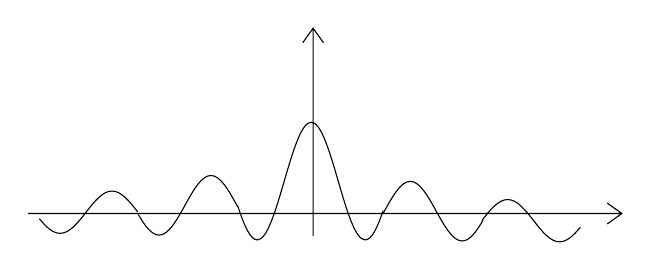
\begin{tikzpicture}[x=0.75pt,y=0.75pt,yscale=-1,xscale=1]
%uncomment if require: \path (0,300); %set diagram left start at 0, and has height of 300

%Shape: Axis 2D [id:dp00630958994675257] 
\draw  (225,191.27) -- (510.99,191.27)(362.25,102) -- (362.25,202) (503.99,186.27) -- (510.99,191.27) -- (503.99,196.27) (357.25,109) -- (362.25,102) -- (367.25,109)  ;
%Shape: Wave [id:dp47979522902139027] 
\draw   (325.99,187.71) .. controls (328.98,196.99) and (332,204) .. (335.35,204) .. controls (340.06,204) and (344.11,190.17) .. (348.35,175.64) .. controls (352.59,161.11) and (356.65,147.27) .. (361.35,147.27) .. controls (366.06,147.27) and (370.11,161.11) .. (374.35,175.64) .. controls (378.59,190.17) and (382.65,204) .. (387.35,204) .. controls (390.43,204) and (393.23,198.07) .. (395.99,189.9) ;
%Shape: Wave [id:dp717311860093465] 
\draw   (278.03,191.74) .. controls (281.23,197.25) and (284.43,201.67) .. (288.03,201.67) .. controls (292.55,201.67) and (296.45,194.66) .. (300.53,187.3) .. controls (304.6,179.94) and (308.5,172.94) .. (313.03,172.94) .. controls (317.55,172.94) and (321.45,179.94) .. (325.53,187.3) .. controls (325.68,187.59) and (325.84,187.87) .. (326,188.16) ;
%Shape: Wave [id:dp528439810330457] 
\draw   (230.36,193.79) .. controls (233.57,197.69) and (236.77,200.83) .. (240.36,200.83) .. controls (244.88,200.83) and (248.78,195.86) .. (252.86,190.64) .. controls (256.94,185.42) and (260.84,180.45) .. (265.36,180.45) .. controls (269.85,180.45) and (273.72,185.35) .. (277.77,190.52) ;
%Shape: Wave [id:dp1416089494426117] 
\draw   (444.08,194.57) .. controls (440.88,200.08) and (437.68,204.5) .. (434.08,204.5) .. controls (429.56,204.5) and (425.66,197.49) .. (421.58,190.14) .. controls (417.51,182.78) and (413.61,175.77) .. (409.08,175.77) .. controls (404.56,175.77) and (400.66,182.78) .. (396.58,190.14) .. controls (396.43,190.42) and (396.27,190.71) .. (396.11,190.99) ;
%Shape: Wave [id:dp9189698618814189] 
\draw   (491,197.87) .. controls (487.79,201.77) and (484.59,204.91) .. (481,204.91) .. controls (476.48,204.91) and (472.58,199.94) .. (468.5,194.72) .. controls (464.42,189.5) and (460.52,184.54) .. (456,184.54) .. controls (451.51,184.54) and (447.64,189.43) .. (443.59,194.61) ;
\end{tikzpicture}
\end{center}

For periodic signals $x(t) = e^{j\omega_0 t}$
$$
e^{j\omega_0 t} \xrightarrow{F} 2\pi \delta(\omega - \omega_0)
$$
\textbf{\textit{Pf.}}
\begin{align*}
	x(t) &= \frac{1}{2\pi} \int_{-\infty}^{\infty} X(j\omega) e^{j\omega t}\text{d}\omega \\
			 &= \frac{1}{2\pi} \int_{-\infty}^{\infty} 2\pi \delta(t) e^{j\omega t} \text{d} \omega \\
			 &= \int_{-\infty}^{\infty} \delta(t) e^{j\omega t}\text{d} \omega \\
			 &= e^{j\omega t}
\end{align*}
\newpage
\subsection*{Properties}
Linearity
$$
\alpha x(t) + \beta y(t) \xrightarrow{F} \alpha X(j\omega) + \beta Y(j\omega)
$$
Time shifting
$$
x(t-t_0) \xrightarrow{F} e^{-j\omega t_0}X(j\omega)
$$
Conjugation
$$
x^*(t) \xrightarrow{F} X^*(-j\omega)
$$
Conjugate symmetry
$$
X(-j\omega) = X^*(j\omega)
$$
If $x(t)$ is real, 我們可以用以下性質證出$e^{-a\left|t\right|} \xrightarrow{F} \frac{a}{a^2+\omega^2}$
\begin{align*}
	Ev \{x(t)\} &\longrightarrow \Re \{X(j\omega)\} \\
	Od \{x(t)\} &\longrightarrow j\Im \{X(j\omega)\} \\
	\because e^{-at}u(t)l &\xrightarrow{F} \frac{1}{a+j\omega} \\
	\therefore e^{-a\left|t\right|} &= 2Ev \{e^{-at}u(t)\} \\
	Ev \{e^{-at}u(t)\}&\xrightarrow{F} \Re \{\frac{1}{a+j\omega}\} = \frac{a}{a^2 - \omega^2} \\
	\Rightarrow e^{-a\left|t\right|} &\xrightarrow{F} \frac{2a}{a^2 - \omega^2}
\end{align*}
Differentiation
$$
\frac{\text{d}x(t)}{\text{d}t} \xrightarrow{F} j\omega X(j\omega)
$$
Integration
$$
\int_{-\infty}^{t} x(\tau)\text{d}\tau \xrightarrow{F} \frac{1}{j\omega}X(j\omega) + \underbrace {\pi X(0) \delta(\omega)}_{\text{\color{red} dc term of integration}}
$$
Time scaling
$$
x(at) \xrightarrow{F} \frac{1}{\left|a\right|}X(\frac{j\omega}{a}) \\
$$
Parseval's relation
$$
\int_{-\infty}^{\infty} \left|x(t)\right|^2 \text{d}t = \frac{1}{2\pi} \int_{-\infty}^{\infty} \left|X(j\omega)\right|^2 \text{d} \omega
$$
\newpage

\subsection*{Covolution property}
The Fourier Transform of LTI system impulse response $h(t)$
$$
H(jk\omega_0 t) = \int_{-\infty}^{\infty} h(t) e^{-jk\omega_0t} \text{d}t
$$
If the outpus is $y(t)$ then
$$
Y(j\omega) = X(j\omega)H(j\omega)
$$
在 time domain 上做 convolution 會在 frequent domain 上做相乘
$$
x(t)*h(t) \xrightarrow{F} X(j\omega)H(j\omega)
$$
\subsection*{Multiplication property}
在 time domain 上做相乘會在frequent domain 上做 convolution
$$
x(t)y(t) \xrightarrow{F} \frac{1}{2\pi}S(j\omega)*P(j\omega)
$$
\subsection*{Scalar in time domain}
在 time domain 乘上變數會是 frequent domain 的微分
$$
tx(t) \xrightarrow{F} j\frac{\text{d}}{\text{d}\omega}X(j\omega)
$$
\subsection*{LCCDE(Linear constant coefficient DE)}
System describe by differential equation
$$
\sum_{k=0}^{N}a_k\frac{\text{d}^ky(t)}{\text{d}t^k} = \sum_{k=0}^{M}b_k\frac{\text{d}^kx(t)}{\text{d}t^k}
$$
By Fourier transform
\begin{align*}
	\sum_{k=0}^{N}a_k(j\omega)^kY(j\omega) &= \sum_{k=0}^{M}b_k(j\omega)^kX(j\omega) \\ 
	H(j\omega) = \frac{Y(j\omega)}{X(j\omega)} &= \frac{\sum_{k=0}^{M}b_k(j\omega)^k}{\sum_{k=0}^{N}a_k(j\omega)^k}
\end{align*}

\end{document}
